\chapter{Sensor tests}

%\section{Digital}
%    \subsection{Interface tests}
%    \subsection{Software tests}

\section{Power}
    \subsection{LDO stabilisation}
        Voltage after LDO was measured in time, to calculate delay between power enable and measurement start. Time graph is shown in the figure \ref{LDO_rise_time}. Delay was estimated to be around \SI{1}{\second}.

        \begin{figure}[H]
            \centering
            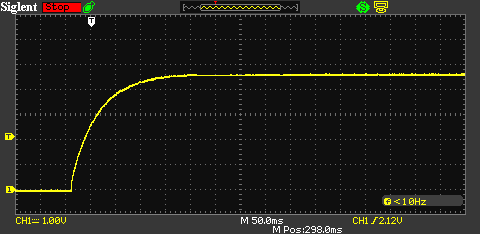
\includegraphics[width=0.8\paperwidth]{img/07/rise_time.png}
            \caption{LDO rise time}
            \label{LDO_rise_time}
        \end{figure}

    \subsection{Power consumption}
        Current drawn during readout is about \SI{25}{\milli\ampere} at \SI{5}{\volt} rail, so power consumption of the sensor equals \SI{0.125}{\watt}.

\section{Current source}
    Current source was tested on HP 34970A - 6 1/2 digit multimeter, with 200 PLC enabled.

    \subsection{Noise}
        Noise of current source was measured for long period of time, taking sufficient number of samples. Results (\ref{Current_Stability}) shows that noise floor is below specifications for this meter.

        \begin{figure}[H]
            \centering
            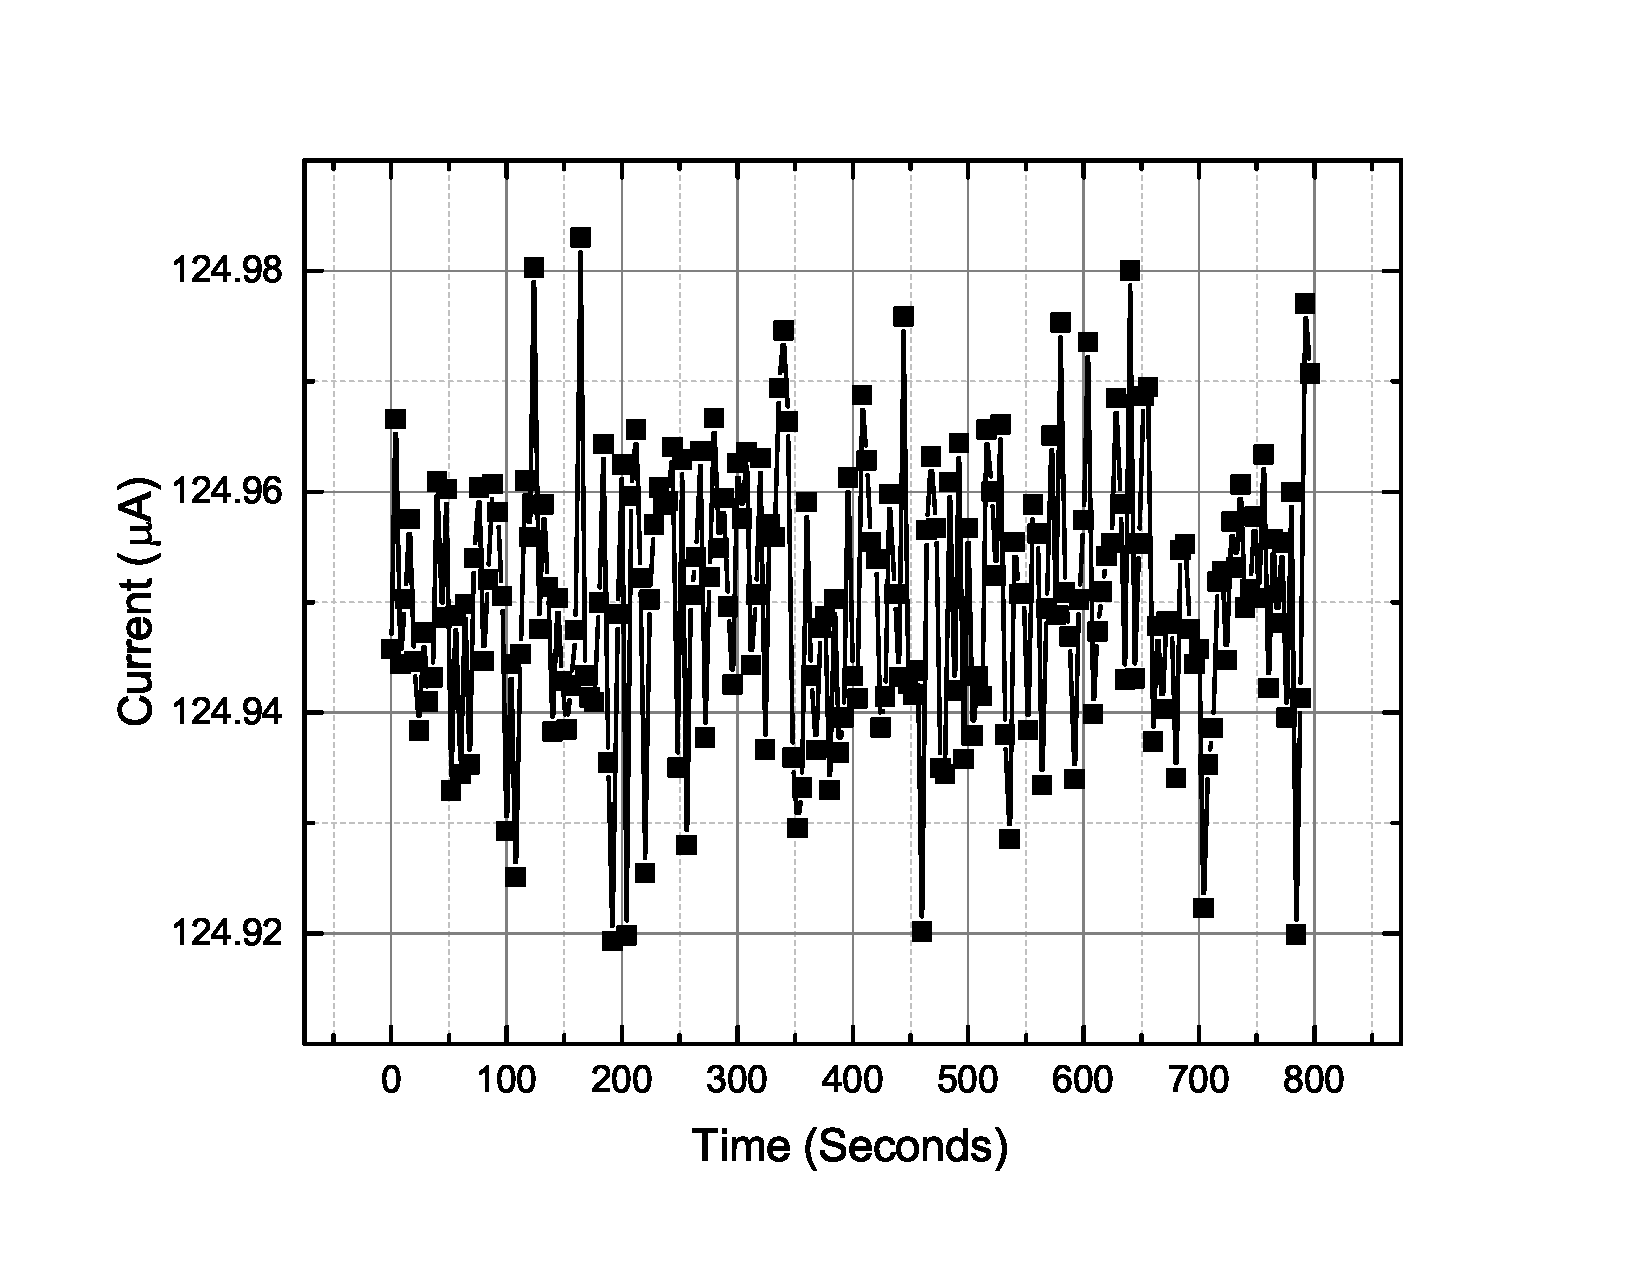
\includegraphics[width=0.6\paperwidth]{img/07/current_time.eps}
            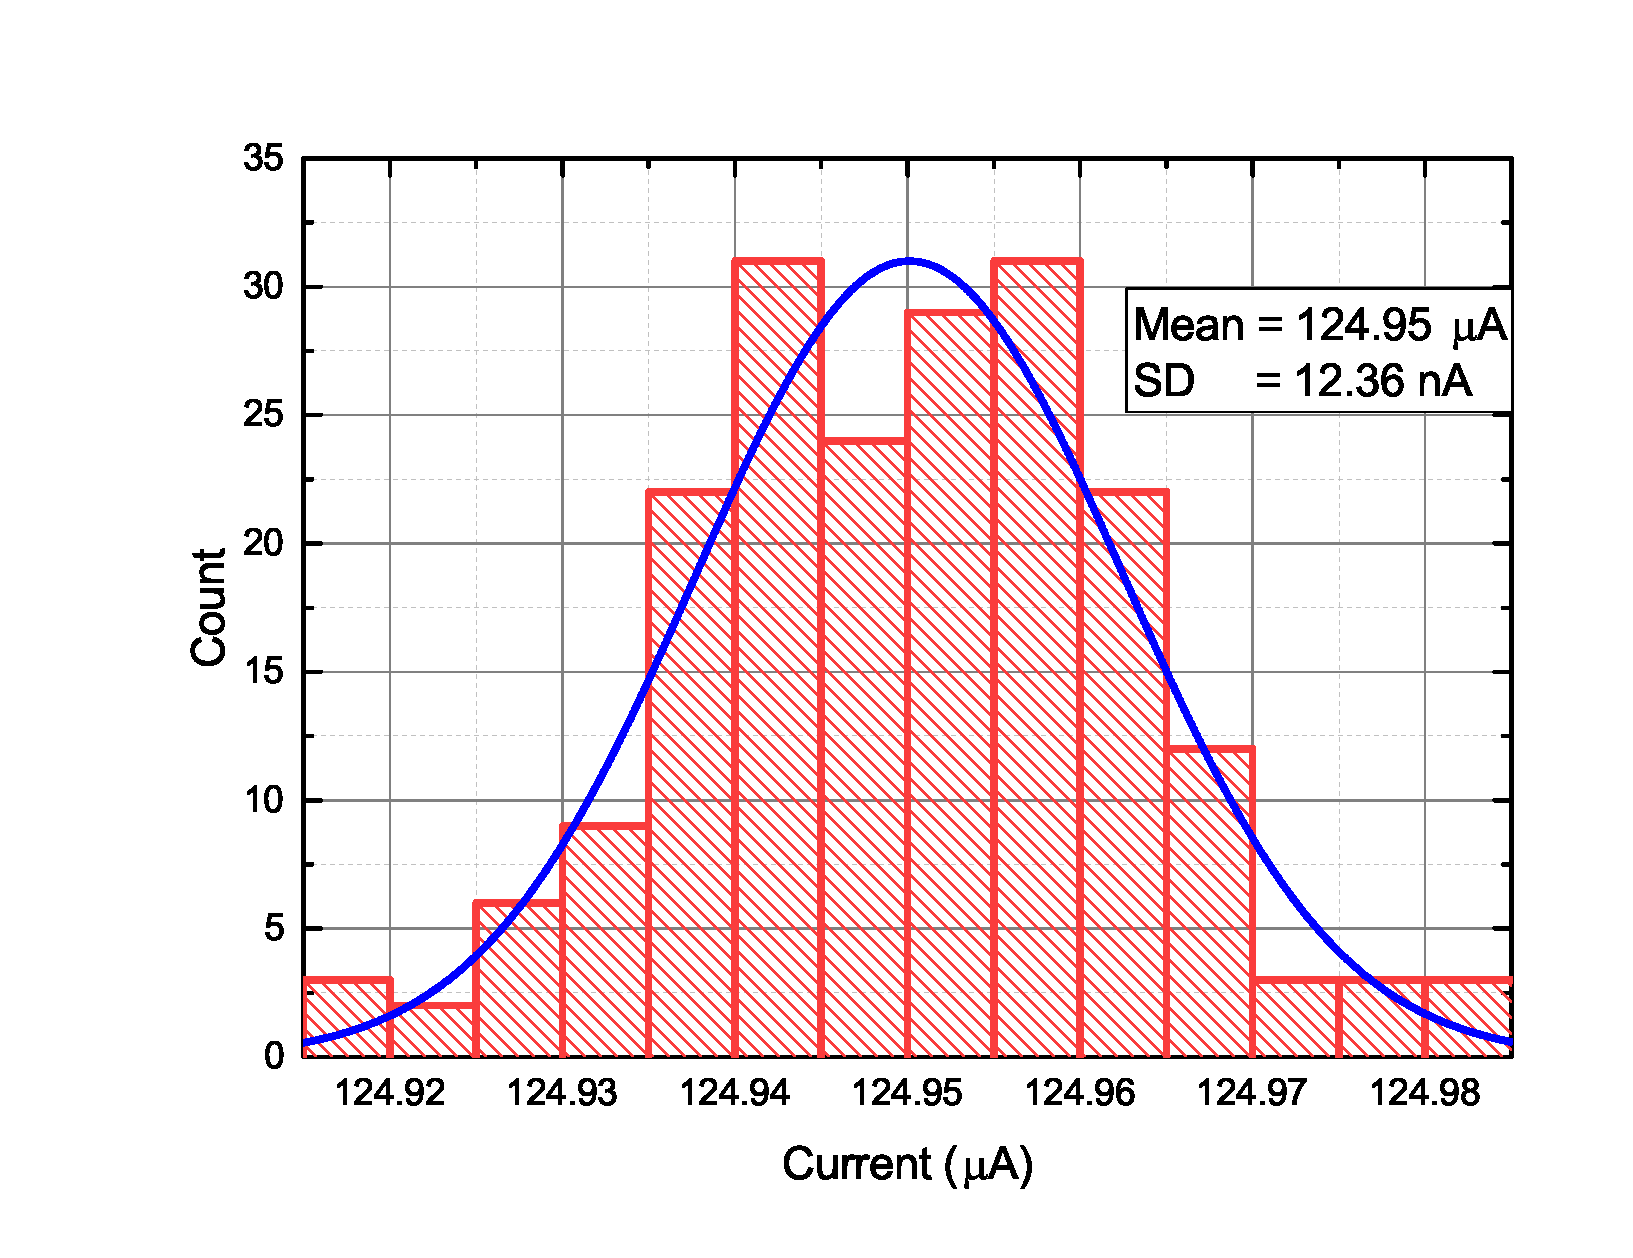
\includegraphics[width=0.6\paperwidth]{img/07/current_hist.eps}
            \caption{LDO rise time}
            \label{Current_Stability}
        \end{figure}

    \subsection{Load range}
        Output load was changed in identical manner as in simulation, to tests its fidelity. Simulation and build model shown same range and stability - confirming the design. Current source works as intended for loads between \SI{1.4}{\kilo\ohm} and \SI{22.5}{\kilo\ohm} (figure \ref{Current_sensor_output_characteristics}).
        \begin{figure}[H]
            \centering
            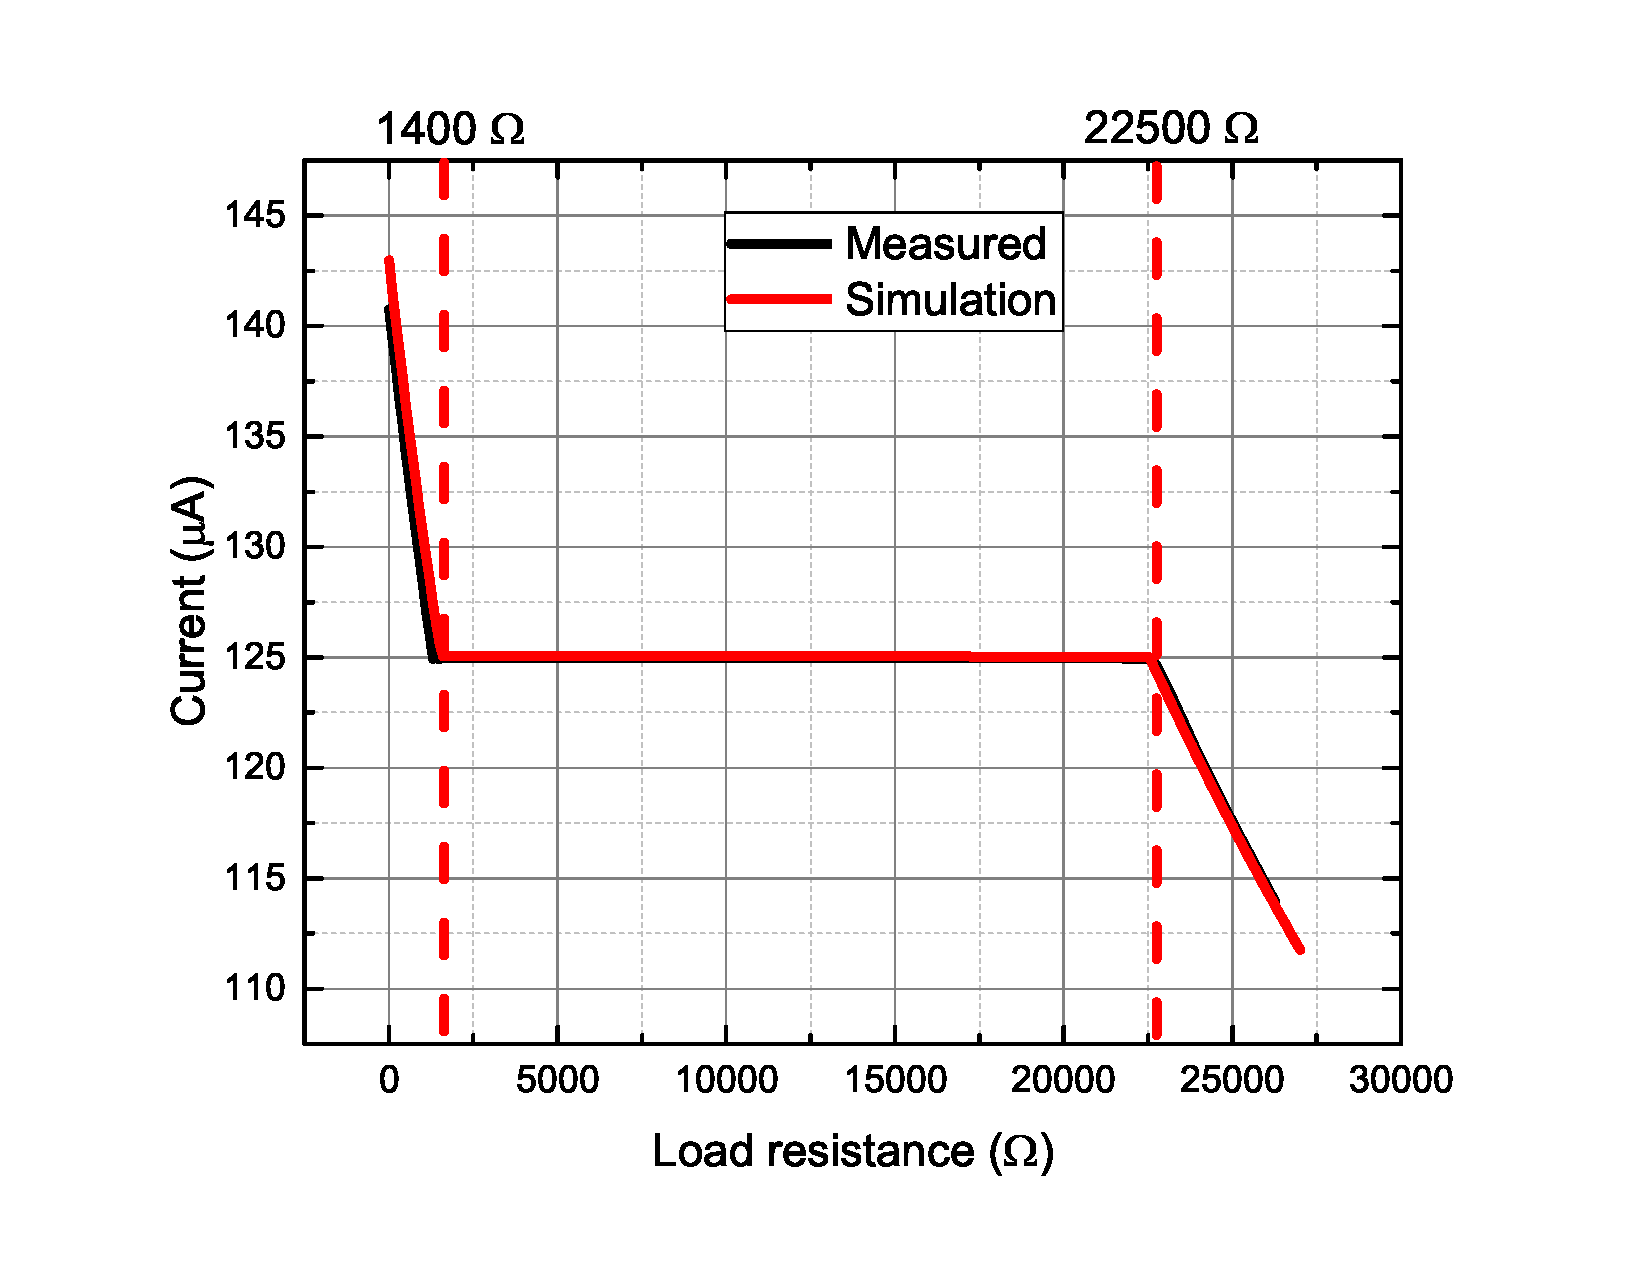
\includegraphics[width=0.9\paperwidth]{img/07/output_resistance.eps}
            \caption{Current sensor output characteristics}
            \label{Current_sensor_output_characteristics}
        \end{figure}

    \subsection{Temperature stability}
        Temperature was swept from $20$ to \SI{70}{\degreeCelsius}, no detectable changes were measured by available meter, therefore it is assumed that current source changes lower than about \SI{20}{\nano\ampere} in this temperature range.

\section{MOS settling}
    After enabling measurement channel for threshold voltage it takes a lot of time to fully stabilize its value. Instead of pre-enabling, same time method was used. ADC takes measurement of threshold voltage at precisely specified time after enabling power. In the figure \ref{MOS_settling} 10 runs of measured voltage vs time are plotted, proving this method is stable within \SI{20}{\uV}.

    \begin{figure}[H]
        \centering
        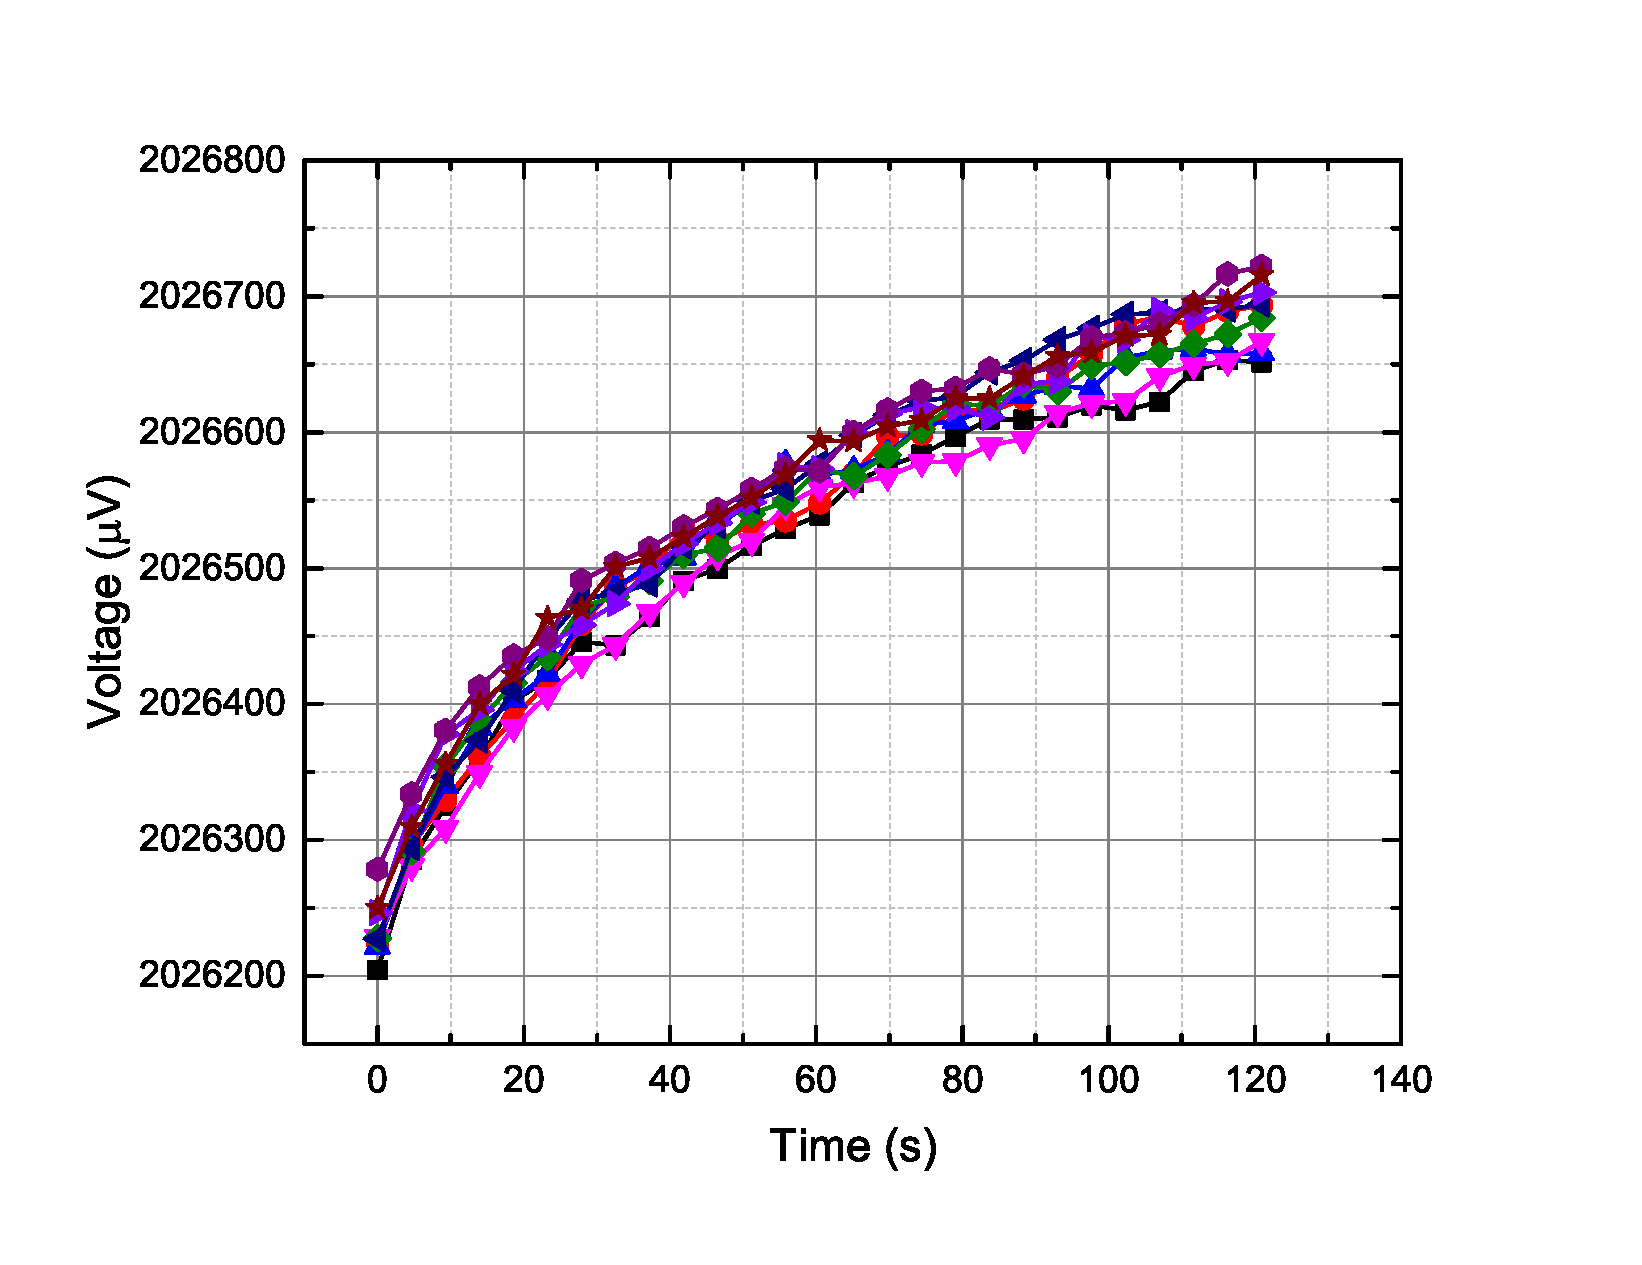
\includegraphics[width=0.8\paperwidth]{img/07/MOS_settling.eps}
        \caption{10 runs of MOS voltage setting}
        \label{MOS_settling}
    \end{figure}

\section{Measurement noise}
    Most important noise figure is system noise - ADC reading noise floor during nominal work.

    Because even smallest temperature changes cause ADC reading to shift (due to threshold/diode voltage shift) this efect had to be eliminated to measure noise. For this purpose DC notch filter was used in post-processing, to eliminate any DC bias during measurement. Sampling frequency of ADC was its nominal rate of \SI{0.25}{\hertz}. Example of filtration is shown in the figure \ref{notch_DC_example}.

    \begin{figure}[H]
        \centering
        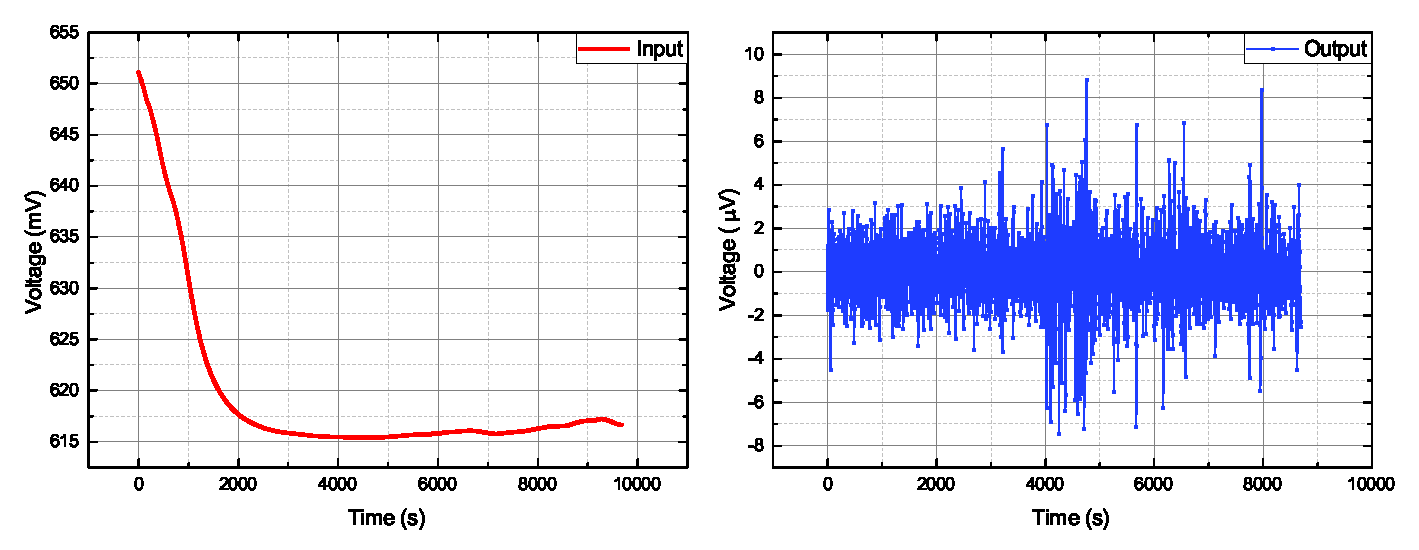
\includegraphics[width=0.8\paperwidth]{img/07/filterBeforeAfter.eps}
        \caption{Input and output of DC notch filter}
        \label{notch_DC_example}
    \end{figure}

    \subsection{Diode}
        \begin{figure}[H]
            \centering
            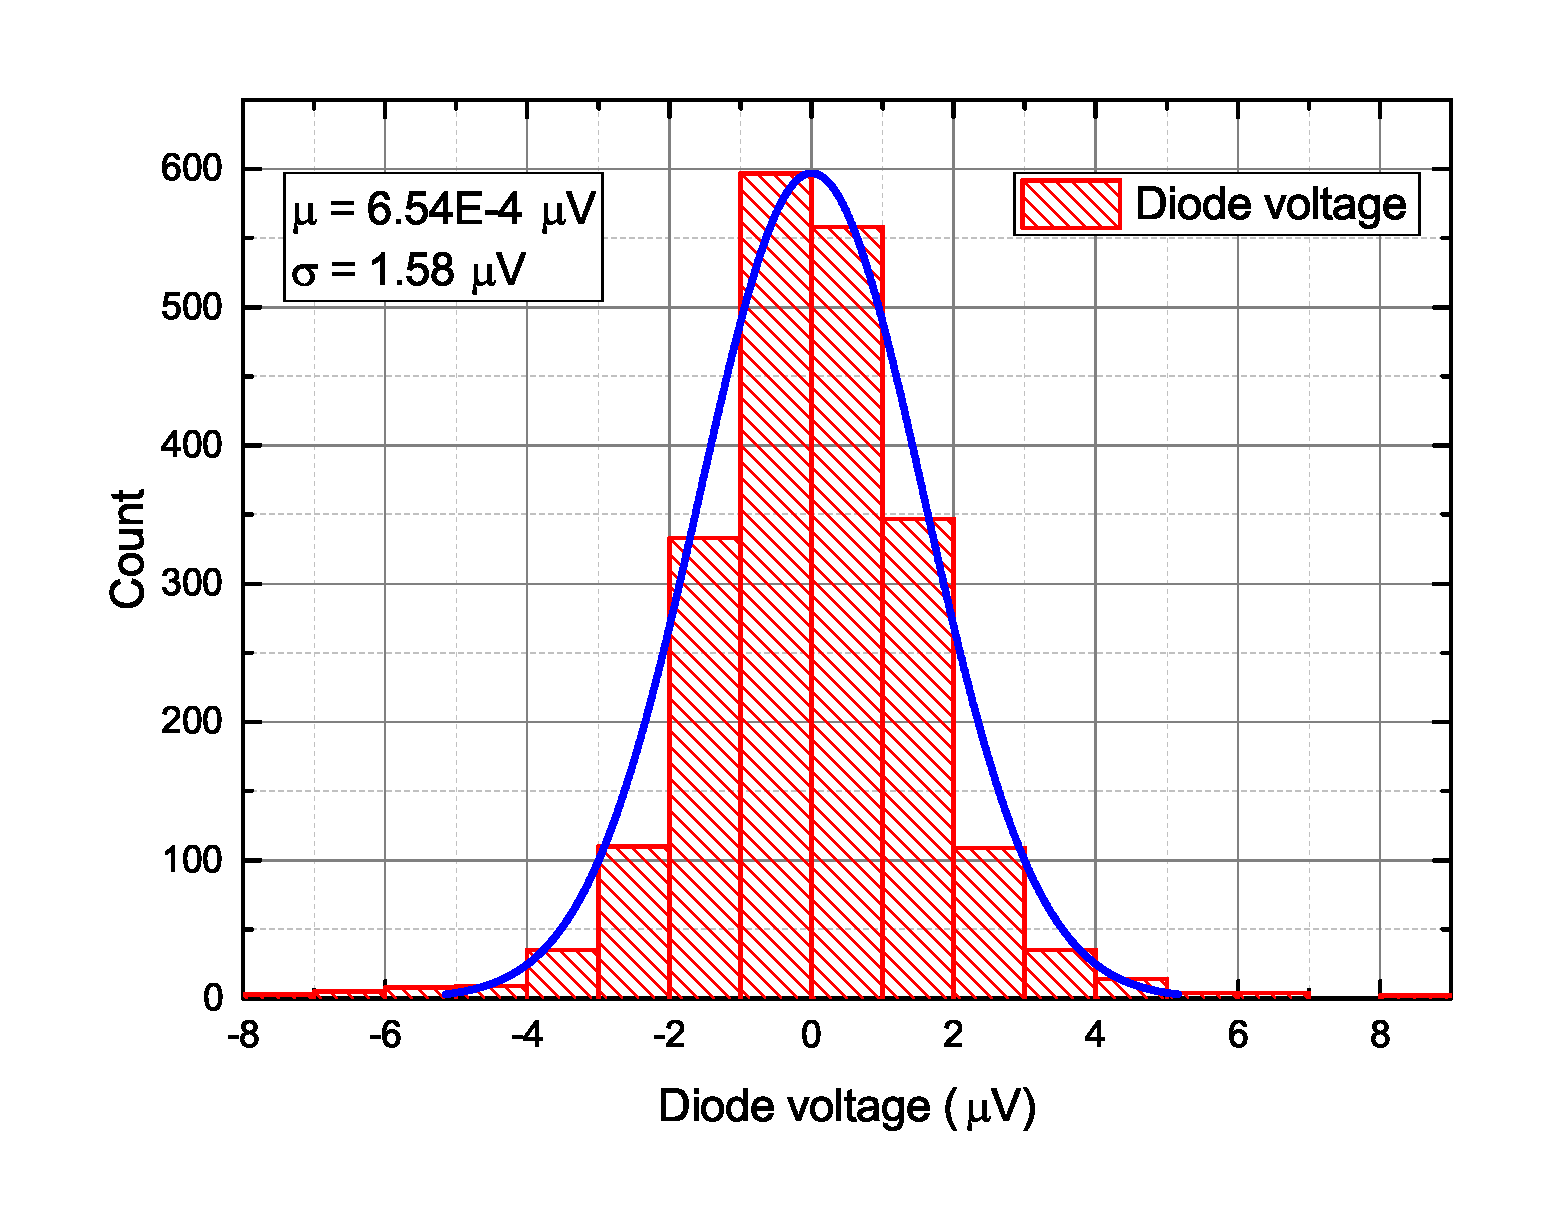
\includegraphics[width=0.8\paperwidth]{img/07/diodeVoltage.eps}
            \caption{Measured noise on body temperature channel}
        \end{figure}

        Noise on temperature measurement channel have standard deviation of $\SI{1.58}{\uV}$
    \subsection{Threshold voltage}
        \begin{figure}[H]
            \centering
            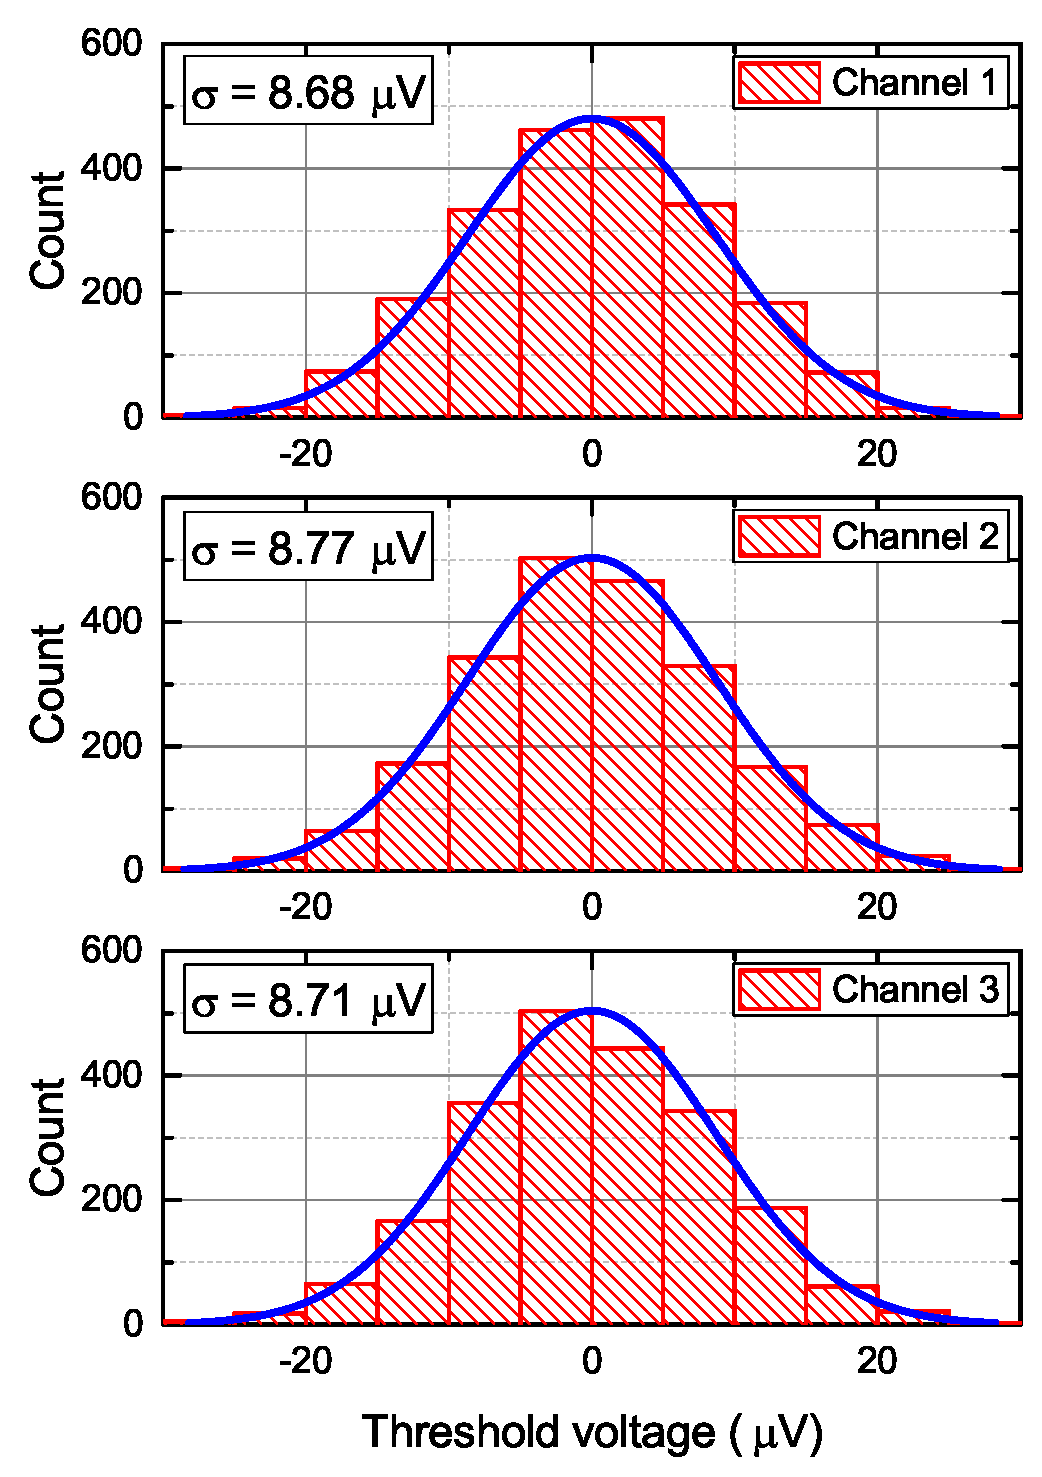
\includegraphics[width=0.6\paperwidth]{img/07/thresholdVoltageHistograms.eps}
            \caption{Measured noise on body temperature channel}
        \end{figure}

        Noise on threshold voltage measurement channel have standard deviations of \SI{8.68}{\uV}, \SI{8.77}{\uV}, \SI{8.71}{\uV}.



    \subsection{Interpretation}
        Because the only difference between temperature and threshold voltage channels is semiconductor itself, source of noise can be estimated from significant difference between them.

        Dependence between threshold voltage and drain current for this type of transistor was measured by M. Gumiela:
        $$I_D~[\mu A] = 410.376 \cdot (V_{TH} - 1.56457)^2 \text{~~~~~~Source: \ref{CD4007_p-MOSFET_transfer}}$$
        $$\frac{\textit{d}}{\textit{d}V_{TH}} I_D= 820.75 \cdot (-1.56 + V_{TH}) = \SI{439.46}{\uA/V} \text{~~~@ operating point}$$
        $$\textit{d}I_d = \SI{3.82}{\nA}$$
        Estimated equivalent current source have RMS value of $I_{N~RMS} = \SI{3.82}{\nA}$.

        This value is the same order of magnitude as calculated: reference voltage LT1634 have low-frequency noise of $U_N = \SI{15}{\uV}$ [TODO], this value is sensed directly across series resistor, therefore $I_{NOISE} = U_N/R = \SI{1.5}{\nA}$. Left part of the noise can origin from different part of the circuit, thermal and shot noise etc. % Noise output from LTSpice:



\section{Temperature characteristics}
    By sweeping temperature from \SI{0}{\degreeCelsius} up to \SI{75}{\degreeCelsius} temperature dependency charts were obtained for the device.

    \subsection{Diode}
        Diode response (figure \ref{Body_diode_temperature_dependency}) is almost ideally linear.
        \begin{figure}[H]
            \centering
            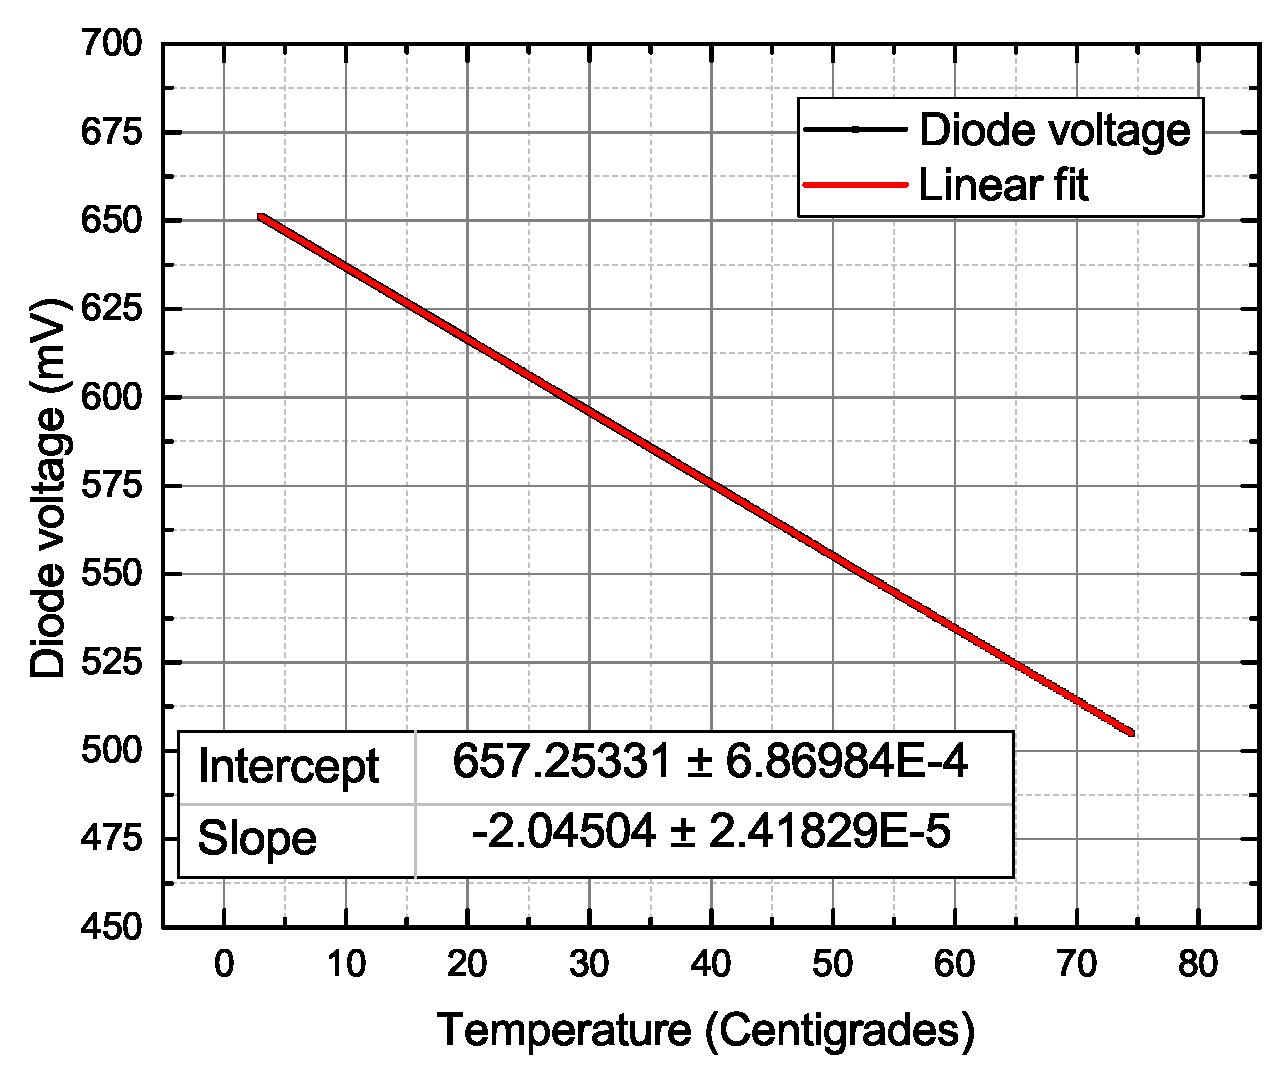
\includegraphics[width=0.6\paperwidth]{img/07/diodeVsTemperature.eps}
            \caption{Body diode temperature dependency}
            \label{Body_diode_temperature_dependency}
        \end{figure}


    \subsection{Threshold voltage}
        Threshold voltage (figure \ref{threshold_voltage_temperature_dependency}) tends to be non-linear, but quadratic equation can be fitted to it. Equation used: $V_{TH} = a \cdot t^2 + b \cdot t + c$, fitted parameters are shown in table \ref{vth_fit_params}.
        \begin{figure}[H]
            \centering
            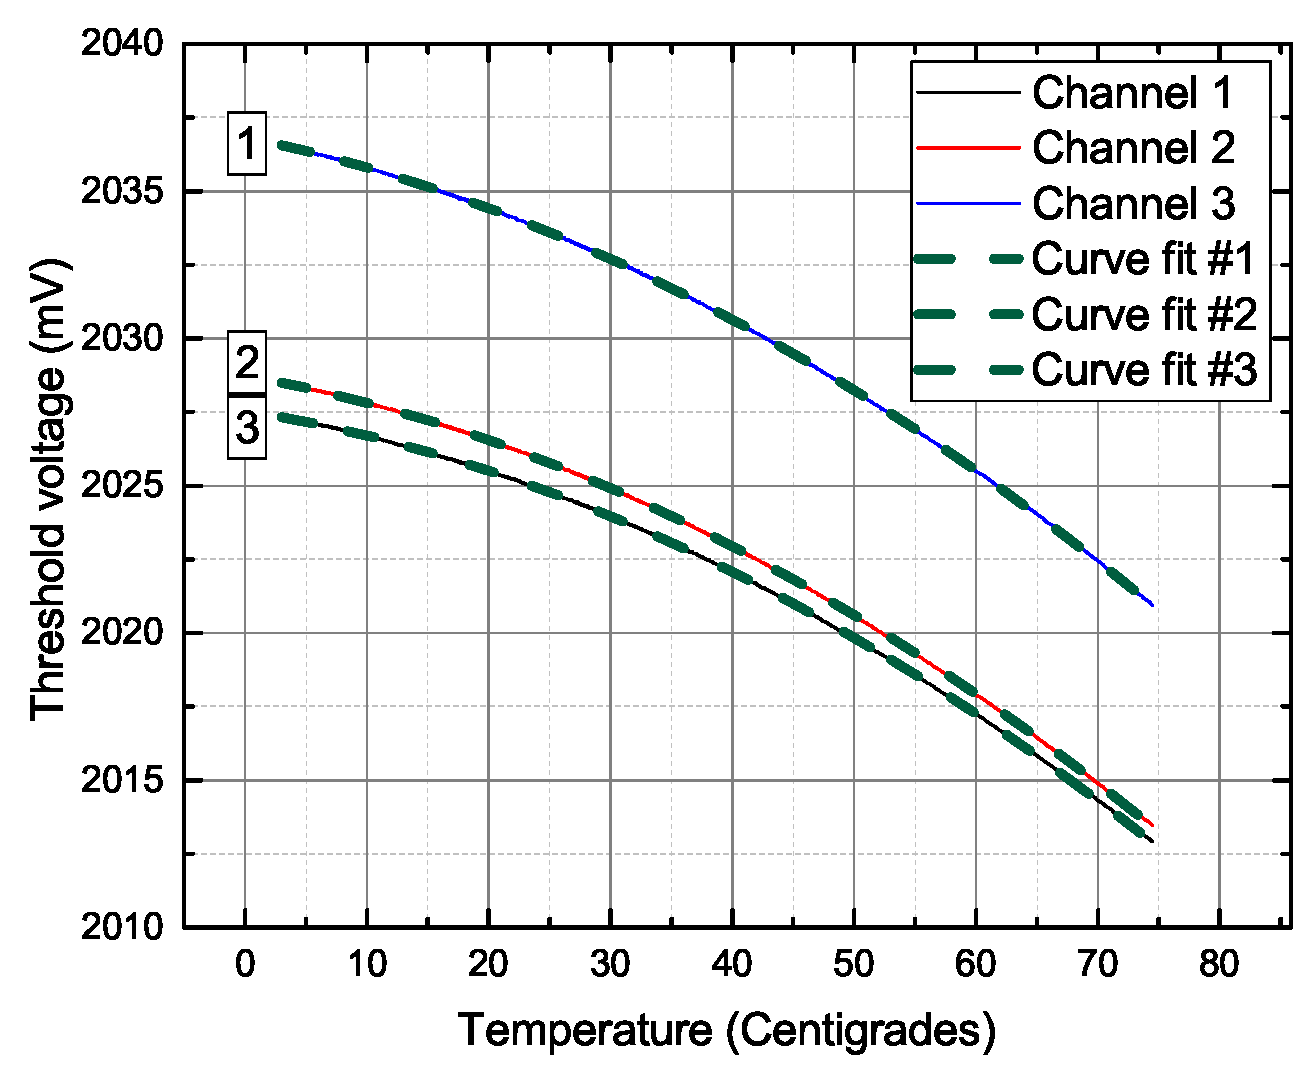
\includegraphics[width=0.6\paperwidth]{img/07/thresholdVoltageTemperatureDependency.eps}
            \caption{Threshold voltage temperature dependency}
            \label{threshold_voltage_temperature_dependency}
        \end{figure}

        \begin{table}[H]
            \begin{center}
                \begin{tabular}{c|c|c|c}
                    Channel & a & b & c \\ \hline
                    ch 1 & $-0.00174~\pm~1.17011e-6$ & $-0.06692~\pm~8.33551e-5$ & $2027.53424~\pm~0.00125$ \\
                    ch 2 & $-0.00176~\pm~1.07318e-6$ & $-0.07437~\pm~7.64496e-5$ & $2028.72804~\pm~0.00114$ \\
                    ch 3 & $-0.00169~\pm~1.12071e-6$ & $-0.08736~\pm~7.98355e-5$ & $2036.83689~\pm~0.00119$ \\
                \end{tabular}
            \end{center}
            \caption{Temperature compensation results}
            \label{vth_fit_params}
        \end{table}

\section{Temperature compensation stability}
    The sensor should be compensated for temperature, with assumption that temperature characteristic curves will not change during irradiation.

    During temperature sweep data was gathered, and post-processed applying thermal compensation (given by charts \ref{Body_diode_temperature_dependency} and \ref{threshold_voltage_temperature_dependency}). In full sensing range, sensor output shifts of maximum $\SI{104}{\uV}$, which reflects to TID measurement accuracy of about \SI{\pm 1}{\rad}. Take note, TID dependency was not tested, but assumed according to \cite{COTSMosfetsGarcia}. Detailed accuracies are listed in table \ref{Temperature_compensation_results}.


    \begin{figure}[H]
        \centering
        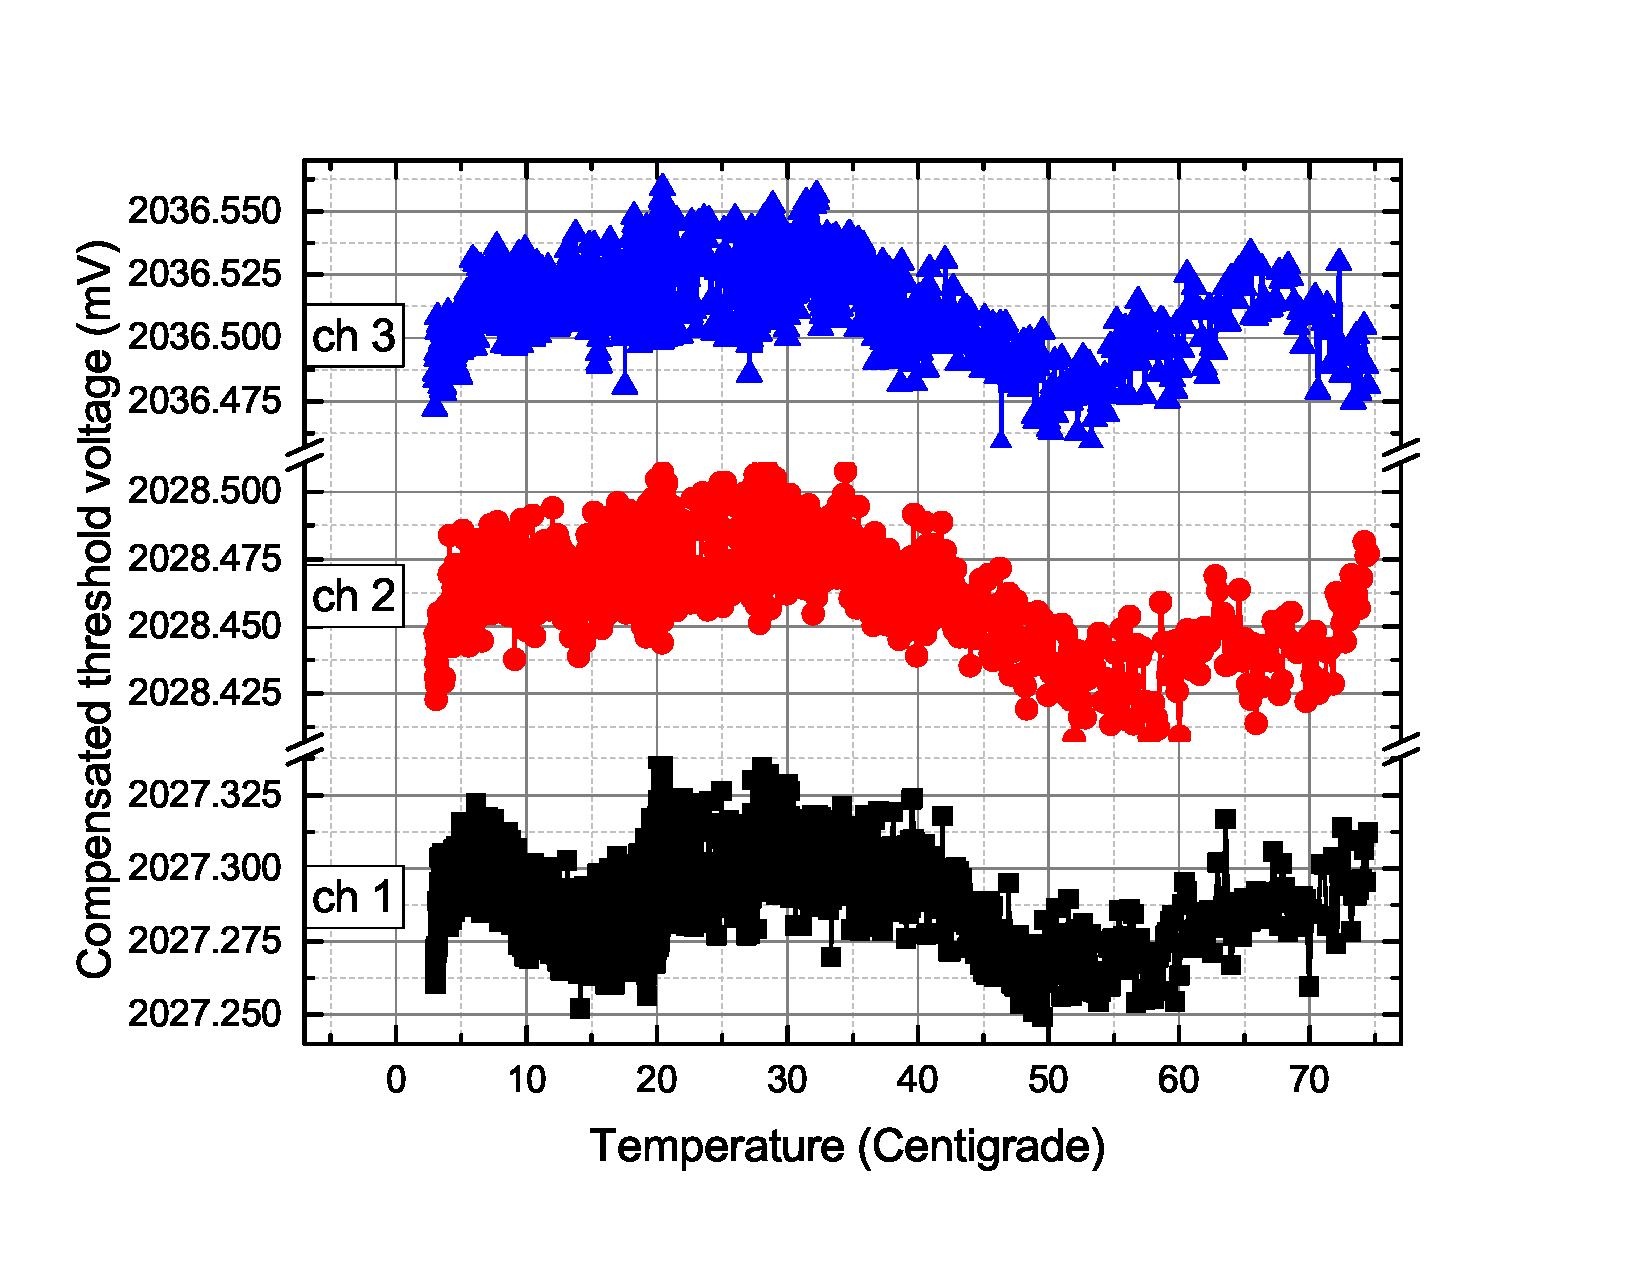
\includegraphics[width=0.8\paperwidth]{img/07/compensatedThresholdVoltage.eps}
        \caption{Threshold voltage temperature compensation}
        \label{threshold_voltage_temperature_compensation}
    \end{figure}

    \begin{table}[H]
        \begin{center}
            \begin{tabular}{c|c|c|c}
                Channel & Standard deviation & Maximum difference & Accuracy ($3~\sigma$) \\ \hline
                ch 1 & \SI{15.13}{\uV} & \SI{89.40}{\uV} & \SI{\pm~0.0108}{\gray} = \SI{\pm~1.08}{\rad} \\
                ch 2 & \SI{16.27}{\uV} & \SI{103.24}{\uV} & \SI{\pm~0.0109}{\gray} = \SI{\pm~1.09}{\rad} \\
                ch 3 & \SI{15.36}{\uV} & \SI{101.26}{\uV} & \SI{\pm~0.0103}{\gray} = \SI{\pm~1.03}{\rad} \\
            \end{tabular}
        \end{center}
        \caption{Temperature compensation results}
        \label{Temperature_compensation_results}
    \end{table}
